\documentclass[11pt]{article}
\usepackage{hyperref}
\usepackage{amsthm}
\usepackage{amsmath}
\usepackage{amsfonts}
\usepackage{tikz}
\usepackage{ wasysym }
\usepackage{fancyvrb}
\usetikzlibrary{arrows.meta,positioning}


\newtheorem{example}{Example}


\author{Group 1:  Nicholas Jacob}
\title{Homework 3 Advanced Analytics and Metaheuristics}

\begin{document}
\maketitle

\begin{enumerate}
\item Team Building
\begin{enumerate}
\item 
\item
\end{enumerate}
\item Outdoor Grilling



 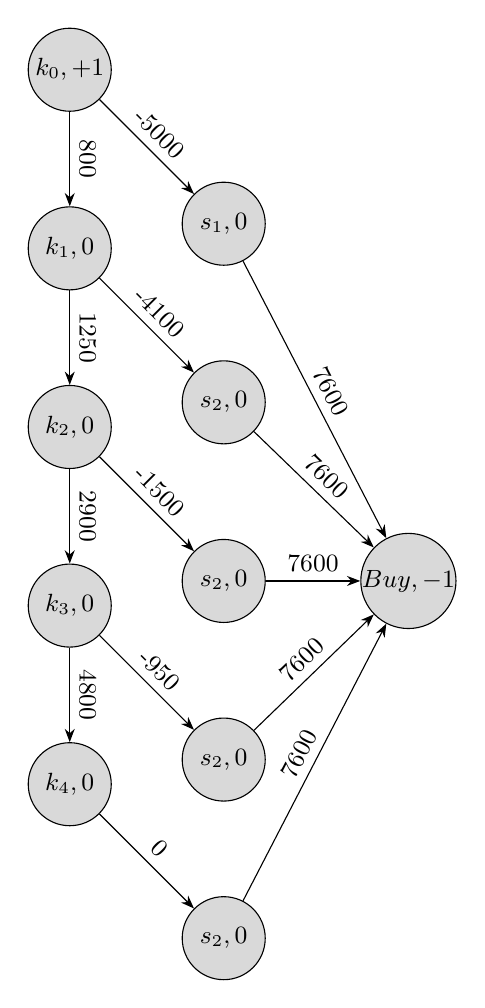
\begin{tikzpicture}[
      mycircle/.style={
         circle,
         draw=black,
         fill=gray,
         fill opacity = 0.3,
         text opacity=1,
         inner sep=0pt,
         minimum size=30pt,
         font=\small},
      myarrow/.style={-Stealth},
      node distance=1.2cm and 1.2cm
      ]
      \node[mycircle] (k0) {$k_0, +1$};
      \node[mycircle,below =of k0] (k1) {$k_1, 0$};
      \node[mycircle,below=of k1] (k2) {$k_2, 0$};
	 \node[mycircle,below=of k2] (k3) {$k_3, 0$};
	 \node[mycircle,below=of k3] (k4) {$k_4, 0$};
	 \node[mycircle,below right=of k0] (s1) {$s_1, 0$};
	 \node[mycircle,below=of s1] (s2) {$s_2, 0$};
	\node[mycircle,below=of s2] (s3) {$s_2, 0$};
	\node[mycircle,below=of s3] (s4) {$s_2, 0$};
	\node[mycircle,below=of s4] (s5) {$s_2, 0$};

      \node[mycircle,right=of s3] (buynew) {$Buy, -1$};

    \foreach \i/\j/\txt/\p in {% start node/end node/text/position
      k0/k1/800/above,
      k1/k2/1250/above,
      k2/k3/2900/above,
      k3/k4/4800/above,
      k0/s1/-5000/above,
      k1/s2/-4100/above,
      k2/s3/-1500/above,
      k3/s4/-950/above,
      k4/s5/0/above,
	 s1/buynew/7600/above,
	 s2/buynew/7600/above,
	 s3/buynew/7600/above,
	 s4/buynew/7600/above,
	 s5/buynew/7600/above}
       \draw [myarrow] (\i) -- node[sloped,font=\small,\p] {\txt} (\j);


    \end{tikzpicture}
\item Here is my flow model:


 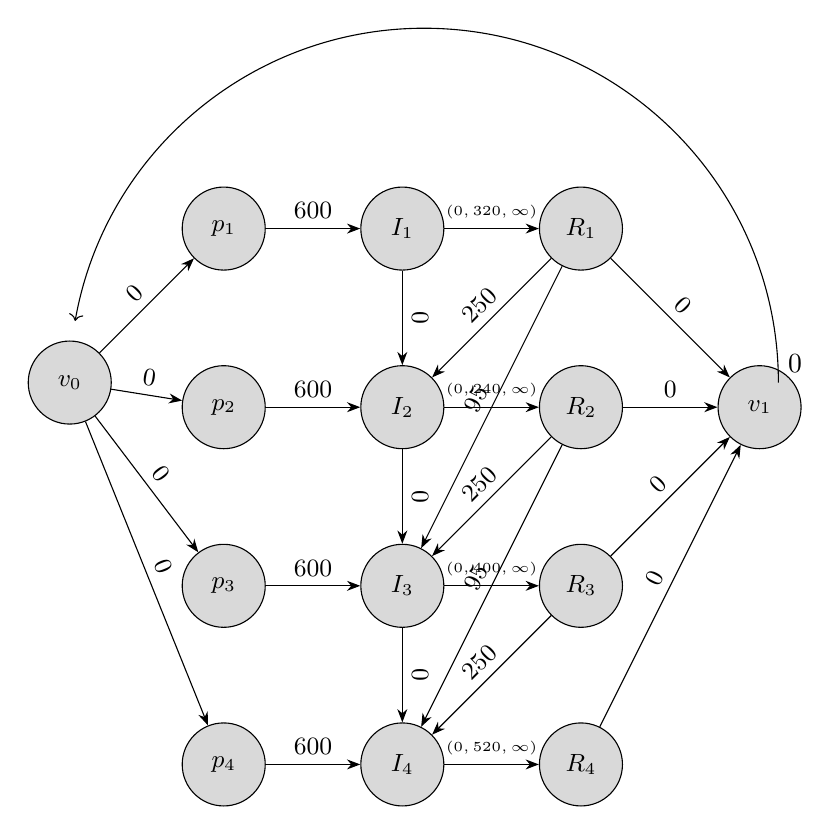
\begin{tikzpicture}[
      mycircle/.style={
         circle,
         draw=black,
         fill=gray,
         fill opacity = 0.3,
         text opacity=1,
         inner sep=0pt,
         minimum size=30pt,
         font=\small},
      myarrow/.style={-Stealth},
      node distance=1.2cm and 1.2cm
      ]
      \node[mycircle] (v0){$v_0$};
      \node[mycircle,above right =of v0] (p1){$p_1$};
      \node[mycircle,below=of p1] (p2) {$p_2$};
	 \node[mycircle,below=of p2] (p3) {$p_3$};
	 \node[mycircle,below=of p3] (p4) {$p_4$};
      \node[mycircle,right=of p1] (i1) {$I_1$};
      \node[mycircle,below=of i1] (i2) {$I_2$};
	 \node[mycircle,below=of i2] (i3) {$I_3$};
	 \node[mycircle,below=of i3] (i4) {$I_4$};
      \node[mycircle,right=of i1] (r1) {$R_1$};
      \node[mycircle,below=of r1] (r2) {$R_2$};
	 \node[mycircle,below=of r2] (r3) {$R_3$};
	 \node[mycircle,below=of r3] (r4) {$R_4$};      
      \node[mycircle,right=of r2] (v1) {$v_1$};



    \foreach \i/\j/\txt/\p in {% start node/end node/text/position
      v0/p1/0/above,
	 v0/p2/0/above,
      v0/p3/0/above,
	 v0/p4/0/above,
      p1/i1/600/above,
      p2/i2/600/above,
      p3/i3/600/above,
      p4/i4/600/above,
	r1/i2/250/above,
	r1/i3/95/above,
	r2/i3/250/above,
	r2/i4/95/above,
	r3/i4/250/above,
	r1/v1/0/above,
	r2/v1/0/above,
	r3/v1/0/above,
	r4/v1/0/above,
	i1/i2/0/above,
	i2/i3/0/above,
	i3/i4/0/above}
       \draw [myarrow] (\i) -- node[sloped,font=\small,\p] {\txt} (\j);

	\draw[myarrow] (i1) -- node[sloped, font = \tiny, above] {$(0,320,\infty)$} (r1);
\draw[myarrow] (i2) -- node[sloped, font = \tiny, above] {$(0,240,\infty)$} (r2);
\draw[myarrow] (i3) -- node[sloped, font = \tiny, above] {$(0,400,\infty)$} (r3);
\draw[myarrow] (i4) -- node[sloped, font = \tiny, above] {$(0,520,\infty)$} (r4);

	\draw[->] (9,0) node[above right,style={-Stealth}]{0} arc  (0:170:4.5) ;

    \end{tikzpicture}

Here is my model file:

{\small \VerbatimInput{group1_HW3_p3.mod}}

Here is my data file:

{\small \VerbatimInput{group1_HW3_p3.dat}}

Here is my output:

\includegraphics[width = .9\textwidth]{output_p3.png}

We look to be purchasing new tires for both the needs of the first two races, 320 and 200 respectively.  This is the maximum number of tires needed.  We use the normal service on 280 tires from the first race and quick on the other 40.  In second race we use the normal service on 120 but quick fix 120.  For the third race we quick fix all 400 tires used.  We end up with exactly the number of tires needed in the fourth race.  Total cost is \$490 000.

\item Dunder Mifflin

\end{enumerate}



\end{document}
